% Worksheet W1 – The W-Seminar at a glance (1 page)
% Übersetzen: latexmk -xelatex ws-w1-seminar-overview.tex
% ============================================================
% ab-vorlage.tex – gemeinsame Vorlage der Arbeitsblätter
% englisch/12/w-seminar-time/arbeitsblaetter/  (W-Seminar "Time")
% Übersetzen mit:  latexmk -xelatex <datei>.tex   (oder zweimal xelatex)
% Gestaltung wie englisch/13/questions-on-the-text/arbeitsblaetter/ab-vorlage.tex,
% Antwortplatz-Makros (8-mm-Linien) wie informatik/10/java/arbeitsblaetter/ab-vorlage.tex
% Schriften: Carlito (Fließtext), Poppins (Überschriften)
% ============================================================
\documentclass[10pt,a4paper]{article}
\usepackage[a4paper,top=12mm,bottom=13mm,left=14mm,right=14mm,headsep=4mm,headheight=12pt,footskip=7mm]{geometry}
\usepackage{fontspec}
\setmainfont{Carlito}
\newfontfamily\headfont{Poppins}[UprightFont=* Medium, BoldFont=* Medium]
\newfontfamily\headlight{Poppins Light}
\usepackage{xcolor}
\definecolor{prim}{HTML}{2563EB}
\definecolor{primdark}{HTML}{1E3A8A}
\definecolor{sec}{HTML}{7C3AED}
\definecolor{dusk}{HTML}{171A3F}
\definecolor{brass}{HTML}{D9AB2F}
\definecolor{primtint}{HTML}{EFF6FF}
\definecolor{sectint}{HTML}{F5F3FF}
\definecolor{ink}{HTML}{1E293B}
\definecolor{muted}{HTML}{64748B}
\definecolor{rule}{HTML}{CBD5E1}
\definecolor{good}{HTML}{059669}
\definecolor{goodtint}{HTML}{ECFDF5}
\definecolor{warn}{HTML}{B45309}
\definecolor{warntint}{HTML}{FFFBEB}
\definecolor{bad}{HTML}{B91C1C}
\definecolor{badtint}{HTML}{FEF2F2}
% Farben der Zeit-Dimensionen (wie auf der Website)
\definecolor{dlit}{HTML}{B83280}
\definecolor{dphys}{HTML}{2563EB}
\definecolor{dcs}{HTML}{0F8F84}
\definecolor{dpsy}{HTML}{C26A06}
\definecolor{dlang}{HTML}{7C3AED}
\definecolor{dbey}{HTML}{4B5563}
\color{ink}
\usepackage[most]{tcolorbox}
\usepackage{tikz}
\usetikzlibrary{positioning,calc,arrows.meta,shapes.misc}
\usepackage{enumitem}
\setlist{nosep,leftmargin=1.1em,topsep=1pt}
\setlist[itemize]{label=\textcolor{prim}{\small\textbullet}}
\usepackage{tabularx,array,booktabs,colortbl}
\usepackage{multicol}
\usepackage{fancyhdr}
\usepackage{lastpage}
\usepackage{amssymb}
\usepackage{qrcode}
\usepackage{microtype}
\setlength{\parindent}{0pt}
\setlength{\parskip}{0pt}
\linespread{1.02}

% ---------- Kopf- und Fußzeile ----------
\newcommand{\wskopf}{W-Seminar English · Time · Year 12}
\pagestyle{fancy}
\fancyhf{}
\renewcommand{\headrulewidth}{0pt}
\fancyhead[L]{\footnotesize\headlight\textcolor{muted}{\wskopf}}
\fancyhead[R]{\ifnum\value{page}=1\footnotesize\headlight\textcolor{muted}{Name: \rule{38mm}{0.3pt}\quad Date: \rule{18mm}{0.3pt}}\fi}
\fancyfoot[L]{\scriptsize\textcolor{muted}{edu-mrh.de/englisch/12/w-seminar-time}}
\fancyfoot[R]{\scriptsize\textcolor{muted}{\thepage\,/\,\pageref*{LastPage}}}

% ---------- Titel ----------
% \wstitel{Kürzel}{Titel}{Untertitel}
\newcommand{\wstitel}[3]{%
  \begin{tcolorbox}[enhanced,colback=dusk,colframe=dusk,arc=2mm,boxrule=0pt,
     left=4mm,right=4mm,top=2.2mm,bottom=2.2mm,
     interior style={left color=dusk,right color=primdark}]
    \color{white}{\headlight\footnotesize #1}\\[0.3mm]
    {\headfont\LARGE #2}\\[0.6mm]
    {\small #3}
  \end{tcolorbox}\vspace{1mm}}

% ---------- Boxen ----------
% \begin{wsbox}[Optionen]{Nummer}{Überschrift} ... \end{wsbox}
\newtcolorbox{wsbox}[3][]{enhanced,breakable,colback=white,colframe=rule,boxrule=0.5pt,arc=1.5mm,
  left=2.5mm,right=2.5mm,top=1.3mm,bottom=1.3mm,
  title={\headfont\normalsize\textcolor{white}{\colorbox{prim}{\,#2\,}}\;\textcolor{ink}{#3}},
  coltitle=ink,colbacktitle=white,attach title to upper={\par\vspace{0.6mm}},before skip=1.4mm,after skip=1.4mm,#1}
\newtcolorbox{tintbox}[1][]{enhanced,colback=primtint,colframe=primtint,boxrule=0pt,arc=1.2mm,
  left=2mm,right=2mm,top=1.2mm,bottom=1.2mm,#1}
\newtcolorbox{secbox}[1][]{enhanced,colback=sectint,colframe=sectint,boxrule=0pt,arc=1.2mm,
  left=2mm,right=2mm,top=1.2mm,bottom=1.2mm,#1}
\newtcolorbox{goodbox}[1][]{enhanced,colback=goodtint,colframe=goodtint,boxrule=0pt,arc=1.2mm,
  left=2mm,right=2mm,top=1.2mm,bottom=1.2mm,#1}
\newtcolorbox{warnbox}[1][]{enhanced,colback=warntint,colframe=warntint,boxrule=0pt,arc=1.2mm,
  left=2mm,right=2mm,top=1.2mm,bottom=1.2mm,#1}
\newtcolorbox{badbox}[1][]{enhanced,colback=badtint,colframe=badtint,boxrule=0pt,arc=1.2mm,
  left=2mm,right=2mm,top=1.2mm,bottom=1.2mm,#1}

\newcommand{\kl}[1]{{\headfont\small\textcolor{prim}{#1}}}      % kleine Zwischenüberschrift
\newcommand{\klsec}[1]{{\headfont\small\textcolor{sec}{#1}}}
\newcommand{\klc}[2]{{\headfont\small\textcolor{#1}{#2}}}       % Zwischenüberschrift in Farbe
\newcommand{\plus}{\textcolor{good}{\textbf{+}}\ }
\newcommand{\minus}{\textcolor{bad}{\textbf{–}}\ }
\newcommand{\pfeil}{\textcolor{prim}{$\rightarrow$}\ }
\newcommand{\cb}{\raisebox{-0.2ex}{\textcolor{muted}{$\square$}}\ }   % Ankreuzkästchen

% ---------- Antwortplatz (8 mm, wie informatik/10/java) ----------
\newif\ifloesung
\ifdefined\mitloesung \loesungtrue \else \loesungfalse \fi
\newcommand{\lsgfarbe}{\color{sec}\itshape}
\newlength{\zeilenabstand}\setlength{\zeilenabstand}{8mm}
\tikzset{schreiblinie/.style={draw=black!45,line width=0.35pt}}
% Lücke: \luecke[Breite] / \lsg[Breite]{Text}
\newcommand{\lsg}[2][45mm]{%
  \makebox[#1][l]{\rlap{\raisebox{-0.6ex}{\rule{#1}{0.4pt}}}\ifloesung{\lsgfarbe\small\,#2}\fi}}
\newcommand{\luecke}[1][45mm]{\lsg[#1]{}}
% Lücke bis Zeilenende
\newcommand{\lsgrest}[1]{\leavevmode\unskip\hspace{1.5mm}\ifloesung\rlap{\raisebox{0.8pt}{\lsgfarbe\,#1}}\fi\leaders\hbox{\rule[-0.6ex]{0.5pt}{0.4pt}}\hfill\null\par}
\newcommand{\restzeile}{\lsgrest{}}
\newcommand{\lueckentext}{\linespread{1.5}\selectfont\raggedright}
\newcommand{\schreibzeile}{\rule[-2.8mm]{0pt}{8mm}}
% Schreiblinien: \linien{n} / \lsglinien{n}{Text}; erste Linie eine volle Zeilenhöhe unter der Frage
\newcommand{\lsglinien}[2]{\par\vspace{0.5mm}\noindent\begin{tikzpicture}
  \path (0,0) (\linewidth-0.4pt,-#1\zeilenabstand-1.5mm);
  \foreach \i in {1,...,#1}{\draw[schreiblinie] (0.2pt,-\i\zeilenabstand) -- (\linewidth-0.2pt,-\i\zeilenabstand);}
  \ifloesung\node[overlay,anchor=north west,inner sep=0pt] at (1mm,-\zeilenabstand+1pt+5mm) {\parbox[t]{\linewidth-2mm}{\lsgfarbe\raggedright\setlength{\baselineskip}{\zeilenabstand}\rule{0pt}{5mm}#2}};\fi
  \end{tikzpicture}\par}
\newcommand{\linien}[1]{\lsglinien{#1}{}}


\begin{document}

\wstitel{Worksheet W1 · W-Seminar “Time”}{The seminar at a glance}%
{Three semesters, one Seminararbeit. Keep this page in the front of your folder.}

% ------------------------------------------------------------------ 1
\begin{wsbox}{1}{Your road to the Seminararbeit}
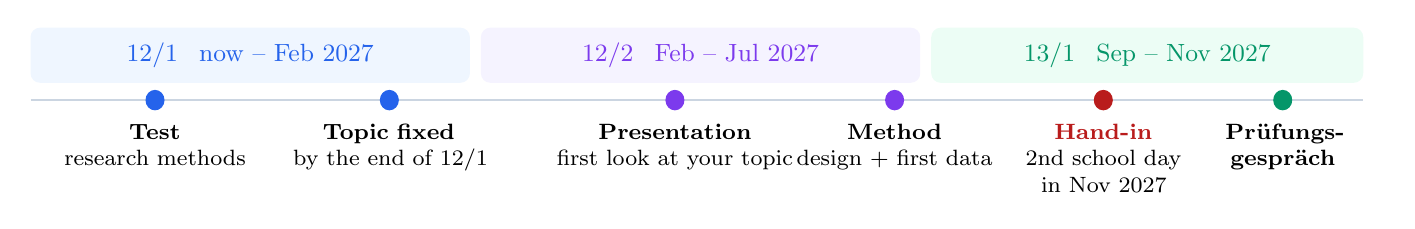
\begin{tikzpicture}[x=0.93mm,y=1mm,font=\footnotesize]
  \def\W{182}
  % Semester bands
  \fill[primtint,rounded corners=1.2mm] (0,0) rectangle (60,7);
  \fill[sectint,rounded corners=1.2mm] (61.5,0) rectangle (121.5,7);
  \fill[goodtint,rounded corners=1.2mm] (123,0) rectangle (\W,7);
  \node[font=\headfont\small,text=prim] at (30,3.5) {12/1 \enspace now – Feb 2027};
  \node[font=\headfont\small,text=sec] at (91.5,3.5) {12/2 \enspace Feb – Jul 2027};
  \node[font=\headfont\small,text=good] at (152.5,3.5) {13/1 \enspace Sep – Nov 2027};
  % Milestones
  \draw[rule,line width=0.6pt] (0,-2.2) -- (\W,-2.2);
  \foreach \x/\col in {17/prim,49/prim,88/sec,118/sec,146.5/bad,171/good}{\fill[\col] (\x,-2.2) circle (1.3);}
  \node[align=center,text width=30mm,anchor=north] at (17,-4) {\textbf{Test}\\research methods};
  \node[align=center,text width=30mm,anchor=north] at (49,-4) {\textbf{Topic fixed}\\by the end of 12/1};
  \node[align=center,text width=30mm,anchor=north] at (88,-4) {\textbf{Presentation}\\first look at your topic};
  \node[align=center,text width=30mm,anchor=north] at (118,-4) {\textbf{Method}\\design + first data};
  \node[align=center,text width=28mm,anchor=north] at (146.5,-4) {\textbf{\textcolor{bad}{Hand-in}}\\2nd school day in Nov 2027};
  \node[align=center,text width=24mm,anchor=north] at (171,-4) {\textbf{Prüfungs-}\\\textbf{gespräch}};
\end{tikzpicture}
\par\vspace{1mm}
{\small In our sessions we alternate between \textbf{methods} (searching, citing, surveys, experiments, statistics, writing) and \textbf{the topic itself} – the many dimensions of time.}
\end{wsbox}

% ------------------------------------------------------------------ 2 + 3
\begin{minipage}[t]{0.49\linewidth}\vspace{0pt}
\begin{wsbox}[height=70mm]{2}{How you are graded}
\renewcommand{\arraystretch}{1.2}
\begin{tabularx}{\linewidth}{@{}l X@{}}
\arrayrulecolor{rule}
\textbf{12/1} & Halbjahresleistung: test + smaller tasks\\
\textbf{12/2} & Halbjahresleistung: presentation + smaller tasks\\\midrule
\textbf{13/1} & \textbf{Seminararbeit} \hfill counts \textbf{×\,2}\\
 & \textbf{Prüfungsgespräch} \hfill counts \textbf{×\,1}\\
\end{tabularx}
\par\vspace{1mm}
{\small\textbf{Prüfungsgespräch}: in our seminar group, led by me. You show that you really understand the content and methods of your paper – expect questions about your working process and how you used AI. Possibly a very short intro first (max.\ 5 min, no full presentation).}
\par\vspace{1mm}
\begin{tintbox}\small Your Abitur certificate lists every part separately: 12/1, 12/2, Seminararbeit, Prüfungsgespräch and their combined result.\end{tintbox}
\end{wsbox}
\end{minipage}\hfill
\begin{minipage}[t]{0.49\linewidth}\vspace{0pt}
\begin{wsbox}[height=70mm]{3}{The Seminararbeit in brief}
\begin{itemize}[itemsep=0.6mm]
\item written \textbf{in English}, the Prüfungsgespräch too
\item about \textbf{10–15 pages} of text (without title page, contents, works cited, appendix)
\item you \textbf{put something to the test}: survey, experiment, measurement or systematic text analysis – and evaluate your own data
\item sources cited in \textbf{MLA style}
\item signed \textbf{declaration of authorship} + \textbf{AI log}
\item format unless announced otherwise: 12\,pt, line spacing 1.5, margins 2.5\,cm
\end{itemize}
\end{wsbox}
\end{minipage}

% ------------------------------------------------------------------ 4
\begin{wsbox}{4}{AI, tools and your own voice}
\begin{minipage}[t]{0.63\linewidth}\vspace{0pt}
AI tools are part of real research – use them, but \textbf{openly}.
\begin{itemize}[itemsep=0.5mm]
\item Keep an \textbf{AI log}: date, tool, what you asked, what you used – \emph{including language polishing}.
\item Never trust an AI reference: check that every source exists and says what you claim.
\item \textbf{Planned:} a supervised writing session later in the seminar. If you want your language to be graded in full, you take part – the text you write there is the reference for your own writing.
\end{itemize}
\end{minipage}\hfill
\begin{minipage}[t]{0.33\linewidth}\vspace{0pt}
\begin{secbox}
\klsec{AI log – one line per use}\par\vspace{1mm}
{\footnotesize
\begin{tabularx}{\linewidth}{@{}l X@{}}
date & 12 Mar 2027\\
tool & chatbot / translator / …\\
task & “Suggest a clearer word order for §2”\\
used & 3 sentences reworded, marked in the text\\
\end{tabularx}}
\end{secbox}
\end{minipage}
\end{wsbox}

% ------------------------------------------------------------------ 5
\begin{wsbox}{5}{Start now}
\begin{minipage}[t]{0.47\linewidth}\vspace{0pt}
\cb Explore the dimensions of time on the website\par\vspace{0.6mm}
\cb Set up a citation tool (e.g.\ Zotero) – save every source right away\par\vspace{0.6mm}
\cb Start a research log: date · what I did · next step\par\vspace{0.6mm}
\cb Note down every idea, however small\par\vspace{0.6mm}
\cb Ask early – about topics, methods, sources
\end{minipage}\hfill
\begin{minipage}[t]{0.5\linewidth}\vspace{0pt}
\kl{Dimensions that interest me – and why}
\linien{3}
\end{minipage}
\end{wsbox}

% ------------------------------------------------------------------ 6
\begin{wsbox}{6}{Questions I still have about the seminar}
\linien{2}
\end{wsbox}

\end{document}
